\section{Evaluation} \label{sec:eval}
In this section, we present the experimental evaluation of 
\siv and \plv. All the experiments are run on an Intel Xeon CPU E5-2640 v6 at 3.00GHz
and an AMD  EPYC 7571 at 2.7GHz.  We aim to address three questions through these
experiments:
%
\begin{itemize}
  %
  \item[Q1.] Is single-instruction validation by itself useful for finding bugs in
  a sophisticated decompiler, even though no context information is used during 
  decompilation?
  %
  \item[Q2.] What fraction of function translations are successfully proven correct
  by \plv, and what is the false alarm rate of the tool?
  %
  \item[Q3.] Given the fact the \plv  comprises of a \compd and \matcher, how is
  the performance of this phase?
  %
  \item[Q4.] Is \plv effective at finding additional potential bugs in a complex 
  lifter like McSema, beyond those found by \siv alone?  We studied this question
  using artificially injected bugs, because all real bugs were caught by \siv.
\end{itemize}

\paragraph{Usefulness of \siv}
The goal here is to validate the lifting of individual \ISA instruction to 
\LLVM sequences using \mcsema. 
Haswell \ISA ISA supports a total of \totalIS instruction variants of which 
\currentIS are formally specified in~\cite{DasguptaAdve:PLDI19}. \mcsema 
supports \mcsemaIS instructions all supported by ~\cite{DasguptaAdve:PLDI19}.
We had to exclude \sivExc instruction variants because of limitations 
of the \LLVM semantics~\cite{LLVMSEMA}, which does not support vector and floating 
points types and associated operations, and various intrinsics 
functions. (However, we do support intrinsics like llvm.ctpop, which is 
pervasively generated in the lifted IR for updating the \reg{pf} flag.) This 
brings us to a total of \sivIS viable instruction variants, and we apply
\TV to each of them individually.
%
Out of the \sivIS translation validations, \sivFail cases fail (hence are bugs) and 
\sivTO timed out. Note that, the solver found conclusive results in all the cases 
(except the timeouts) within a solver timeout of 30 secs. Figure~\ref{fig:solvertime}
shows the distribution of Solver times on tests producing conclusive results. The outliers are
the ones having complex summaries coming out of the lifted IR.

\begin{figure}
    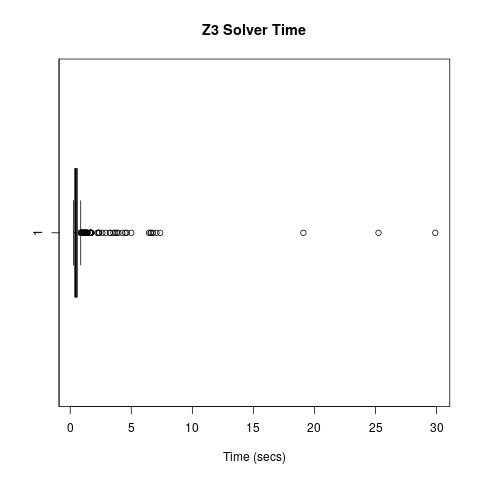
\includegraphics[scale=0.5]{scalable-validation/figs/solver.png}
    \caption{Distribution of \Z solver time} \label{fig:solvertime}
\end{figure}
%%

Timeouts, declared based on a threshold of 24 hrs, correspond to \instr{paddb},
  \instr{psubb}, and \instr{mulq} family of instructions. On further
  investigation, we found that $4$ out of \sivTO timeouts, related to
  \instr{paddb}, \instr{psubb}, are flaky: the \Z solver result toggled between
  \textit{unknown} and \textit{unsat} depending on the order in which other
  unrelated constraints are added (which is a known issue~\cite{ZIssue}). By
  removing the unrelated constraints, \Z concludes them to be equivalent. The
  remaining two cases (related to \instr{mulq}) include solver constraints
  containing bit-vector multiplication which the state-of-the-art SMT solvers
  are not very efficient at reasoning about. However, we manually inspected
  them to check that the generated code fragments are semantically equivalent.
%%

The \sivFail failures were all reported 
as possible bugs~\cite{Suppl} to the \mcsema project, and all \sivFail 
have been confirmed as bugs by the \mcsema developers.
%
The following gives some brief examples of some of the
discrepancies we found.
\begin{itemize}
    \item \instr{xaddq \%rax, \%rbx} expects the operations 
    (1) temp $\leftarrow$ \reg{rax} + \reg{rbx}, (2) \reg{rax} 
    $\leftarrow$ \reg{rbx}, and (3) \reg{rbx} $\leftarrow$ temp, in that 
    order. \mcsema performs the same operation differently as (A) old\_rbx = 
    \reg{rbx}, (B) temp $\leftarrow$ \reg{rax} + \reg{rbx}, (C) \reg{rbx} 
    $\leftarrow$ temp, and (D) \reg{rax} 
    $\leftarrow$ old\_rbx. This will fail to  work when the operands 
    are the same registers.

    \item For instruction \instr{andnps \%xmm2, \%xmm1}, the Intel 
    Manual~\cite{IntelManual} says the implementation should be \reg{xmm1}  
    $\leftarrow$ $\sim$\reg{xmm1} \& \reg{xmm2}, whereas \mcsema 
    interchanges the source operands.
    
    \item For \instr{pmuludq \%xmm2, \%xmm1} instruction, both the higher and 
    lower double-words of the source operands need to multiply, whereas 
    \mcsema multiplies just the lower double-words.
    
    \item For  \instr{cmpxchgl \%ecx, \%ebx}, \mcsema compares the entire $64$-bit 
    \reg{rbx} (instead of just \reg{ebx}) with the accumulator 
    \s{Concat(0x00000000, \reg{eax}}).
    
    \item For \instr{cmpxchgb \%ah, \%al}, the lower $8$-bits of \reg{rax} 
    should be replaced with the higher $8$-bits at the end of the instruction, whereas 
    \mcsema keeps them unchanged.
\end{itemize}

%\todo{Is it mcsema to remill bugs}

%3062 - 159 - 2189
%714
%3062-714
%2348
%
\paragraph{Program-level validation: Success rate and false alarms:}
%
The goal here is to validate the translation of programs, one function at a 
time, using the Matcher strategy (Section~\ref{sec:matcher}). For this purpose, 
we use programs from LLVM-8.0 ``single-source-benchmarks''. The benchmark suite
consists of a total of $102$ programs, of which $11$ cannot be lifted by 
\mcsema due to missing instruction semantics. The remaining programs 
contain $3062$ functions in total. We excluded $714$ functions because  the 
corresponding binary uses floating point instructions which are not supported
in the LLVM formal semantics and so could not be validated using single 
instruction validation. This 
brings us to a grand total of \plvT usable functions which we compiles (using 
both gcc/clang) and feed the binaries to \compd and \mcsema for lifting. The 
length of (inlined) lifted IR functions ranges from $86-21729$, with an average 
of $777$.

Of the \plvT usable functions, our matcher can correctly and formally 
prove the correctness of the translations for \plvP using graph-isomorphism, 
i.e., a success rate of 93\%.
We manually checked the remaining $159$ and found them to be false alarms, with the
following root causes:

\begin{itemize}
 \item \textbf{Phase ordering problem ($~80\%$)}: The normalizer passes are not able to
converge functions into isomorphic graphs mainly because of the order in which
the normalizer passes are applied. We believe that an auto-tuner
(e.g. ~\cite{opentuner2014,HyperOpt13}) exploring
different normalizer pass sequences can greatly improves these results.

 \item \textbf{Difference in Lifting globals ($~20\%$)}: For data section addresses, Mcsema
lifts a global with over-approximated size (as determined by IDA) which need
not be equal to the actual source code size, whereas, we determine the size as
the width of the maximum access across all the instructions accessing that
particular global.  As a result, the lifted global sizes might be different from
\mcsema. The memory-dependence edges that we extract using \LLVM \textit{memoryssa}
analysis depend on the size of the globals and hence the generated graphs will
be different. A more accurate memory analysis might solve these issues.
    
\end{itemize}
%%

%%

Overall, a false alarm rate of about \FPRate is low enough that we believe
our Matcher can be of practical use for validation and testing of a decompiler.


\paragraph{Program-level validation: Performance:}
The performance of this phase is primarily dominated by that of \compd and
\matcher.  We chose to validate single instruction in batch after \plv (thereby
 skipping line 8 in Algorithm~\ref{alg:compd}). Figure~\ref{fig:compdtime} demonstrates
 performance of \compd using a distribution of its runtime. The
 performance depends heavily on the availability of instructions in the Store
 Cache for reuse. For example, even though   ``oourafft/cftmdl'' has the largest number of
 binary instruction (to be lifted to IR), most of the instructions are reused from the
 Store while compositing and hence its composition time is not the most dominating.
 
The amount of reuse depends on the order in which the test functions are
executed.  For example, a bulky function, with many commonly occurring
instructions, if decompiled first (using \compd), will populate  the Store
sufficiently to be reused across other functions.  Even with an
arbitrary order of test execution, the Store reuse is found significant.
Figure~\ref{fig:reuse} shows the distribution of reuse percentage (both across
    \& within functions) for an arbitrary order of lifter execution on \plvT
test-functions.

\begin{figure}
    \includegraphics[scale=0.5]{scalable-validation/figs/reuse.png}
    \caption{Distribution of reuse \% within \& across functions
        for an arbitrary execution sequence \compd 
        on test-subjects (i.e. functions)} \label{fig:reuse}
\end{figure}


\begin{figure}
    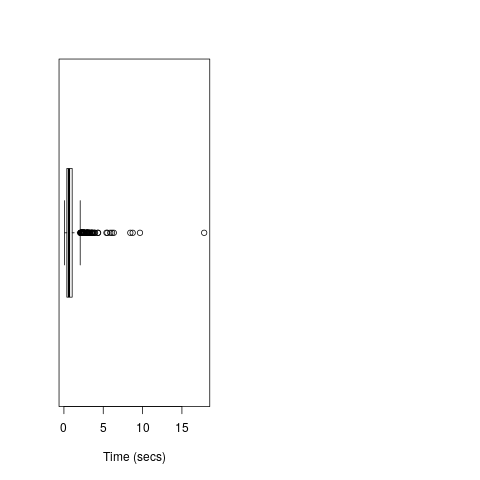
\includegraphics[scale=0.5]{scalable-validation/figs/compdtime.png}
    \caption{Distribution of  \compd time} \label{fig:compdtime}
\end{figure}

The matcher includes includes an algorithm~\cite{Saltz2014} for subgraph-isomorphism
having a complexity of $\Theta(n \times e \times p)$ (worst-case $\mathcal{O}(n^3)$), where $n, e, p$ are
the number of nodes in \GN (or \GNP), the average number of edges per node, and the average
size of the potential-match set $\Phi$ respectively. However, the way we define the initial match set $\Phi$
keeps $p$ pretty low, thereby improving the performance, as shown in Figure~\ref{fig:matchtime}. 
\begin{figure}
    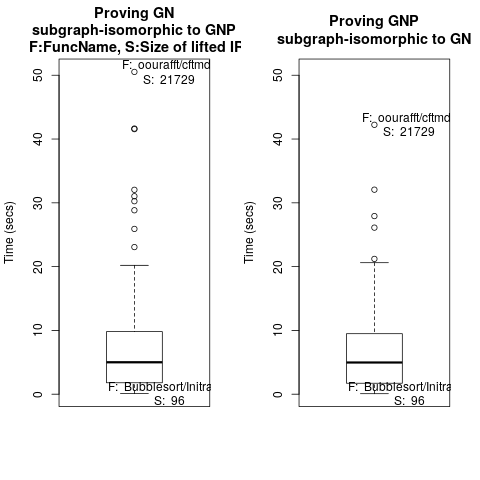
\includegraphics[scale=0.5]{scalable-validation/figs/matchtime.png}
    \caption{Distribution of  \matcher time} \label{fig:matchtime}
\end{figure}


\paragraph{Program-level validation: Effectiveness at finding bugs:}
%
In order to evaluate whether our strategy is effective in finding bugs in lifters like 
McSema, we manually injected bugs in their implementation. The injected bugs 
cover the following aspects of \mcsema's lifting: (1) \emph{Instruction 
lifting}: McSema 
while lifting uses code templates to generate IR sequences for each instruction. 
The injected bug forces the tool to choose wrong templates. The injected bug is 
targeted to affect the translation of $491$ unique instruction mnemonics that 
we collected from the compiled binaries of our evaluation test-suite.   
%
(2) \emph{Inferring data-section access constant}: \mcsema uses information from 
IDA~\cite{IDA} to know if an immediate operand used in data-section access 
instructions is a constant or a memory address. The introduced bug forces 
\mcsema to take the wrong decision.
%
(3) \emph{Maintaining 
correct data dependence among instructions}: The injected bug changes the 
order in which instructions are lifted, causing
data dependences between the dependent instructions to be violated
%
(4) \emph{Correctness of hoisting address computation code}: 
As mentioned earlier, 
\mcsema hoists the address computations of simulated registers back to the function
entry block, to be reused by 
later instructions throughout the function. Our injected bug forces 
the use of incorrect simulated address for general purpose registers and flags.

Each of the above bugs are injected one at a time and in combination and the 
resulting buggy lifter is tested against the \compd on the same evaluation 
test-suite as before. All the injected bugs are correctly detected by the Matcher,
showing that \plv is useful for detecting bugs, not just proving correctness.

Note that only the first of these bugs would be caught by \siv: the binary instruction
semantics would not match with the LLVM IR sequence semantics in that case.
The second case would (in general) produce equivalent semantics between the X86 and
the LLVM IR sequence, and so \siv would not detect the bug.
The third and fourth bugs inherently span multiple instructions, and generate 
wrong code even if the individual instructions are translated correctly, so \siv 
would \emph{not} be able to detect them.
